\chapter{Εισαγωγή}
\label{ch:introduction}
\section{Κίνητρο}
Ο υπολογισμός της απόστασης που διαχωρίζει δύο αντικείμενα στο 
χώρο αποτελεί θεμελιώδες πρόβλημα στον τομέα της Υπολογιστικής
Γεωμετρίας.
Στη ρομποτική, στη σχεδίαση και μηχανική με τη βοήθεια υπολογιστών 
(\tl{CAD} και \tl{CAE}), στις προσομοιώσεις με υπολογιστές και στη γραφική 
υπολογιστών είναι σημαντικό να γνωρίζουμε εάν δύο αντικείμενα, που περιγράφονται 
από μαθηματικά μοντέλα στον τρισδιάστατο χώρο, τέμνονται/συγκρούονται ή βρίσκονται 
σε κοντινή απόσταση.
Για την παρούσα διπλωματική εργασία, εξετάζουμε την περίπτωση όπου τα αντικείμενα
του χώρου περιγράφονται από τριγωνικά πλέγματα (βλ. \ref{sec:triangle_meshes}). 

Στη ρομποτική, για παράδειγμα, η επίλυση του παραπάνω προβλήματος 
είναι απαιτητή για τον σχεδιασμό διαδρομής με την παρουσία εμποδίων
\tl{(path-planning problem)}
\cite{brooks1985subdivision},
\cite{cameron1985study}, 
\cite{canny1986collision}, 
\cite{culley1986collision}.
Επιπλέον, σε εφαρμογές \tl{CAD-CAE} στις οποίες σχεδιάζονται περίπλοκες 
κατασκευές που αποτελούνται από μεγάλο αριθμό εξαρτημάτων, ο εντοπισμός 
σύγκρουσης μεταξύ των εξαρτημάτων είναι απαραίτητος τόσο για τις αναλύσεις 
και δοκιμές των προϊόντων όσο και για την παραγωγή τους 
\cite{boyse1979interference}. 
Στη γραφική με υπολογιστές και συγκεκριμένα κατά την κίνηση των 
αντικειμένων σε μια εικονική σκηνή, όπως στα βιντεοπαιχνίδια και 
στα κινούμενα σχέδια, είναι πιθανό τα αντικείμενα να διεισδύσουν το 
ένα στο άλλο. Αυτή η κατάσταση δεν είναι επιθυμητή όταν με τα 
γραφικά επιδιώκεται η αναπαράσταση ενός ρεαλιστικού κόσμου
\cite{moore1988collision}.
Τέλος, το πρόβλημα υπολογισμού της απόστασης που διαχωρίζει δύο αντικείμενα 
στο χώρο συναντάται και στον τομέα της υπολογιστικής φυσικής για εφαρμογές 
ανάλυσης πεπερασμένων στοιχείων (\tl{FEA}) και προσομοιώσεων 
\cite{khamayseh2007use}.

Η ραγδαία ανάπτυξη όλων των παραπάνω τομέων τα τελευταία χρόνια
και η απαίτηση λεπτομερέστερης περιγραφής των αντικειμένων του
τρισδιάστατου χώρου, κάνουν επιτακτική την ανάγκη για μελέτη
και σχεδιασμό αλγορίθμων ικανών να διαχειριστούν
μεγάλους όγκους δεδομένων εισόδου. Σε αυτή τη διπλωματική εργασία
προτείνουμε αποδοτικούς αλγορίθμους για τον υπολογισμό της απόστασης 
δύο πλεγμάτων στον τρισδιάστατο χώρο.

\section{Περιγραφή του Προβλήματος}
Δοθέντων δύο αντικειμένων στον χώρο, τα οποία περιγράφονται από 
τριγωνικά πλέγματα, το πιο φυσικό μέγεθος για την περιγραφή της 
εγγύτητας μεταξύ τους είναι η Ευκλείδεια απόσταση. 
Δηλαδή, το μήκος του μικρότερου ευθυγράμμου τμήματος που ενώνει 
τα δύο αντικείμενα. Σε περίπτωση που τα αντικείμενα συγκρούονται 
η απόσταση τους είναι μηδέν.

\begin{figure}[h]
    \centering
    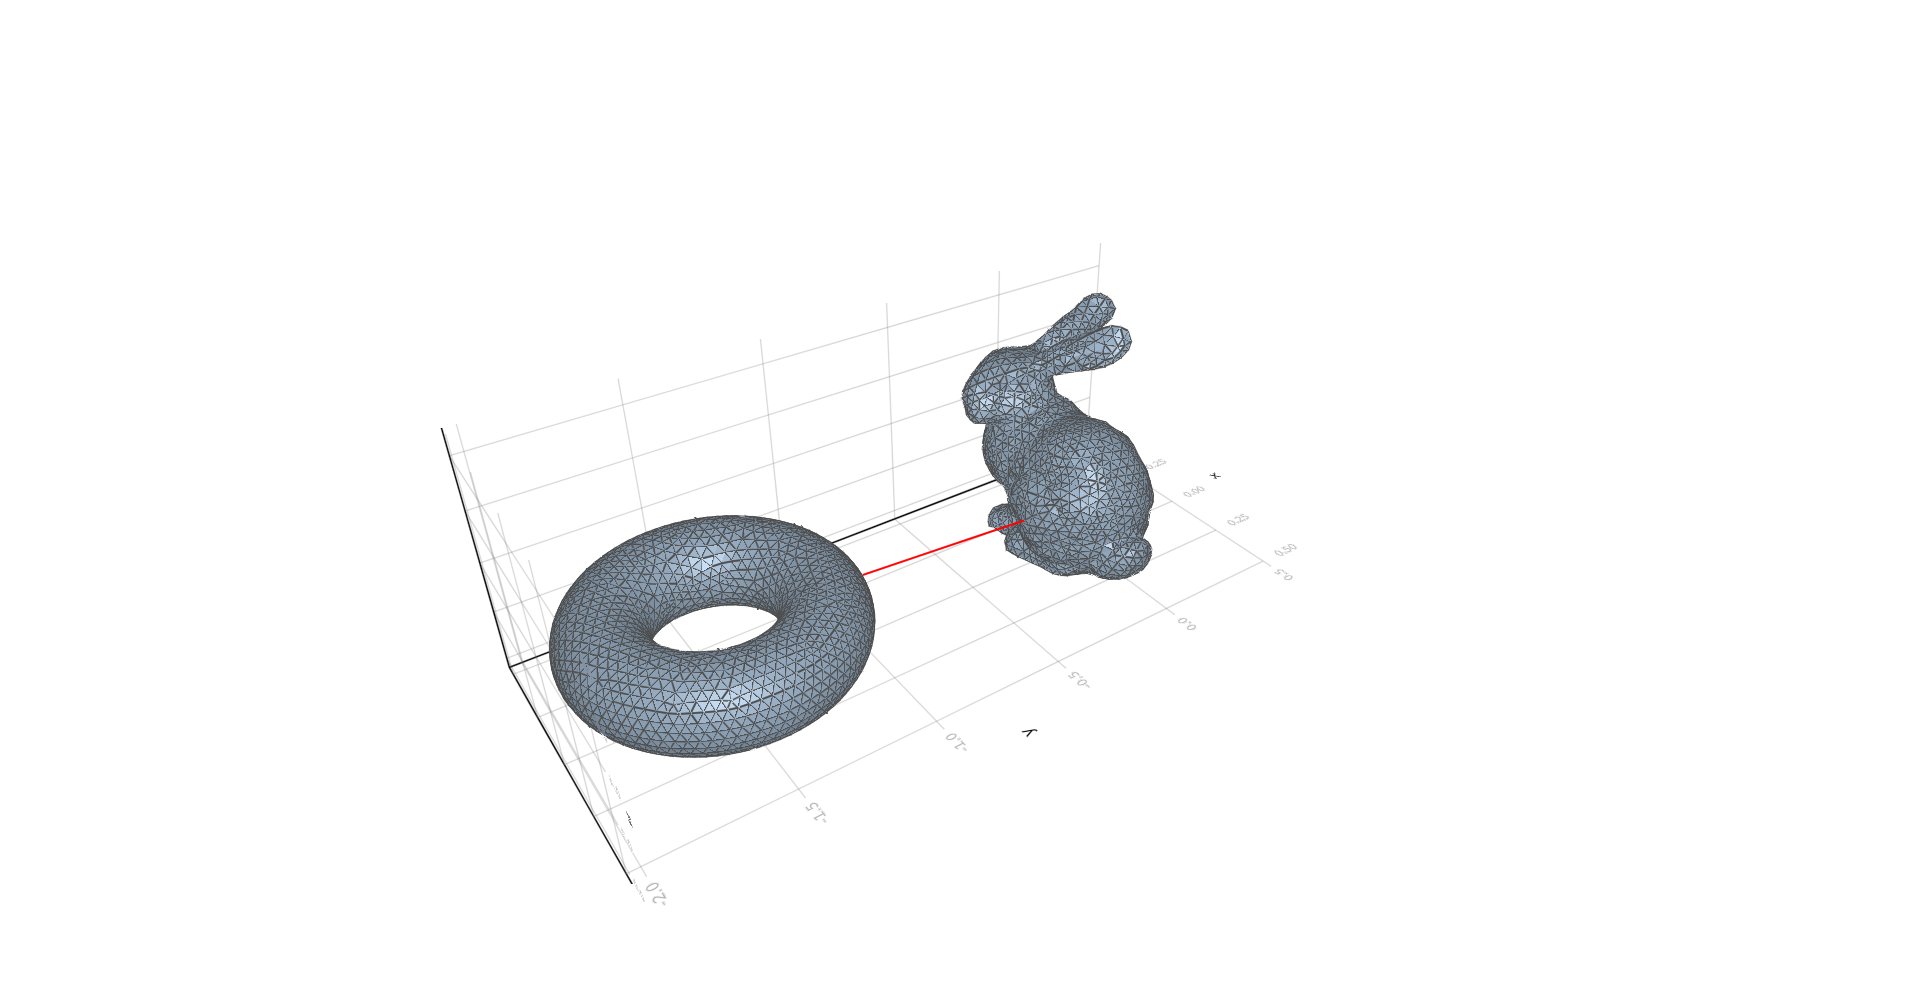
\includegraphics[width=\textwidth]{problem_visualisation.png}
    \caption[Οπτική Αναπαράσταση του Προβλήματος]{
        Ευκλείδεια Απόσταση δύο Τριγωνικών Πλεγμάτων - 
        Το κόκκινο ευθύγραμμο τμήμα αναπαριστά την Ευκλείδεια
        απόσταση ενός Τόρου και του \tl{Stanford Bunny}.  
    }
\end{figure}

Με τον ίδιο ακριβώς τρόπο ορίζεται και η Ευκλείδεια απόσταση 
μεταξύ δύο τριγώνων στον τρισδιάστατο χώρο. 
Σχεδιάζοντας μια τέτοια ρουτίνα (βλ. \ref{subsec:tria_distance}) 
τότε μπορούμε να δώσουμε έναν εναλλακτικό ορισμό του προβλήματος
και ταυτόχρονα έναν αλγόριθμο που το επιλύει: 

\begin{definition}
    Έστω δύο αντικείμενα του τρισδιάστατου χώρου που περιγράφονται 
    από τριγωνικά πλέγματα. Επιπλέον, έστω τα σύνολα $X$, $Y$ που 
    αποτελούνται από τα τρίγωνα των δύο πλεγμάτων, αντίστοιχα, και 
    $tria\_dist(x,y)$ η ρουτίνα που υπολογίζει την Ευκλείδεια απόσταση
    δύο τριγώνων $x$, $y$.
    Η Ευκλείδεια απόσταση $d$ των δύο τριγωνικών πλεγμάτων είναι
    \[ d = \min_{\forall x \in X, \forall y \in Y} tria\_dist(x,y) \]    
\end{definition}

Ο τετριμμένος αλγόριθμος, που βασίζεται στον ορισμό, υπολογίζει την απόσταση 
κάθε πιθανού ζεύγους τριγώνων και επιλέγει την ελάχιστη. Τέτοιοι αλγόριθμοι 
εξαντλητικής αναζήτησης περιγράφονται στο \ref{sec:exhaustive_search}, όμως
είναι αδύνατο να χρησιμοποιηθούν σε πραγματικές εφαρμογές. O λόγος είναι η μεγάλη
υπολογιστική τους πολυπλοκότητα της τάξης $\bigO(N \cdot M)$ (όπου $N$, $M$ το 
πλήθος των τριγώνων των συνόλων $X$, $Y$ αντίστοιχα).

\section{Στόχοι της Διπλωματικής Εργασίας}
Η συνεισφορά της διπλωματικής εργασίας είναι η ακόλουθη:
\begin{itemize}
    \item Σχεδιάζουμε μια δενδρική δομή δεδομένων που ανήκει στην 
    οικογένεια των Ιεραρχιών Οριοθετικών Όγκων (\tl{BVH}). Η δομή 
    αυτή χρησιμοποιείται ως χωρικό ευρετήριο (\tl{spatial indexing}).
    \item Προτείνουμε έναν τρόπο διάσχισης της παραπάνω δομής ώστε 
    να υποστηρίζονται ερωτήματα κοντινότερου γείτονα για χωρικά 
    δεδομένα. Στόχος είναι να ελεγχθεί μόνο ένα μικρό υποσύνολο του 
    χώρου αναζήτησης. Αυτό επιτυγχάνεται με το κλάδεμα (\tl{pruning})
    του δένδρου κατά την αναζήτηση.
    \item Προτείνουμε δύο αλγορίθμους που επιλύουν το πρόβλημα 
    υπολογισμού της Ευκλείδειας απόστασης δύο πλεγμάτων. 
    Οι αλγόριθμοι είναι γενικοί και μπορούν να εφαρμοστούν σε 
    πλέγματα που αποτελούνται από διαφόρων ειδών πολύτοπα (πολύγωνα και 
    πολύεδρα) υπό προϋποθέσεις. Στην εργασία αυτή μελετώνται τα 
    τριγωνικά πλέγματα.
    \item Υλοποιούμε τους αλγορίθμους για συστήματα υψηλής απόδοσης 
    που υποστηρίζουν πολλαπλά νήματα (\tl{multithreading}). 
    Παραλληλοποιούμε τις διαδικασίες κατασκευής του δένδρου και
    αναζήτησης της ελάχιστης απόστασης.
    \item Μετράμε και αναλύουμε την επίδοση των αλγορίθμων μας 
    σε μια σειρά από περιπτώσεις ελέγχου που κατασκευάσαμε. 
\end{itemize}

\section{Διάρθρωση της Διπλωματικής Εργασίας}
Στο \textbf{Κεφάλαιο \ref{ch:introduction}} έγινε μια εισαγωγή στο 
πρόβλημα υπολογισμού της απόστασης δύο πλεγμάτων και παρουσιάστηκαν
τα κίνητρα που οδήγησαν στην υλοποίηση των αλγορίθμων που θα 
παρουσιαστούν. 

Στο \textbf{Κεφάλαιο \ref{ch:theoretical_background}} παρουσιάζεται το 
θεωρητικό υπόβαθρο που απαιτείται από τον αναγνώστη ώστε να κατανοήσει
πλήρως το πρόβλημα και την προτεινόμενη λύση.

Στο \textbf{Κεφάλαιο \ref{ch:related_work}} αναφέρεται η σχετική 
βιβλιογραφία, δηλαδή πώς αντιμετώπισαν άλλοι ερευνητές το ίδιο ή 
παρόμοια προβλήματα. 
Παρουσιάζονται επίσης ομοιότητες και διαφορές
των υπολοίπων προσεγγίσεων σε σχέση με τη δική μας.

Στο \textbf{Κεφάλαιο \ref{ch:methodology}} αναλύεται η μεθοδολογία 
που προτείνουμε και παρουσιάζεται η υλοποίηση των αλγορίθμων μας.

Στο \textbf{Κεφάλαιο \ref{ch:experiments}} παρατίθενται τα αποτελέσματα 
από τα πειράματα που εκτελέσαμε. 
Οι μετρήσεις των πειραμάτων περιλαμβάνουν την εκτίμηση της μετρικής 
κόστους που ορίζεται στην ενότητα \ref{sec:cost_metric} καθώς και τους χρόνους
εκτέλεσης των αλγορίθμων. 

Στο \textbf{Κεφάλαιο \ref{ch:future_work}} σχολιάζονται τα αποτελέσματα
και παρουσιάζονται σκέψεις για μελλοντική επέκταση και βελτίωση των 
ιδεών της παρούσας διπλωματικής εργασίας.
